
\chapter{Specific Requirements}

\section{General}

The requirements will be presented categorized in sections depending on the functionality or the ASW part that shall apply them. Under each section all the requirements are listed, and for a better understanding of the system and better reference to the requirement a global numbering system has been prepared.\\

Each requirement number has the numbering form of "RXX-XX": "R" for requirement followed by four numbers separated by a dash. The first two numbers refer to the group/section each requirement belongs, while the two other numbers are the number of the requirement in the group.\\

Section/group list with the corresponding numbering:
\begin{enumerate}
\item[00] Modes
\item[01] Initialization
\item[02] Commands
\item[03] Telemetry
\item[04] Performance
\item[05] Interface
\item[06] Operation
\item[07] Resource
\item[08] Verification
\item[09] Acceptance testing
\item[10] Documentation
\item[11] Security
\item[12] Portability
\item[13] Quality
\item[14] Reliability
\item[15] Maintainability
\item[16] Safety
\item[17] SW Design and Programming
\end{enumerate}

As the developed ASW is highly constrained by the interacting systems, all following requirements are ranked as essential.

\section{Functional requirements}

\subsection{Modes}

The ASW shall have three different modes. Those modes are INIT, NORMAL and SAFE. The transitions between the modes are shown in \abb{fig:modes}.\\


\begin{figure}
\centering
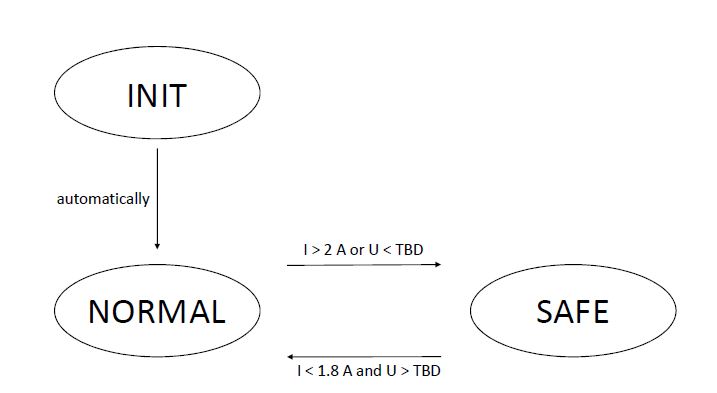
\includegraphics[scale=0.8]{modes.PNG}
\caption{Transitions between modes.}
\label{fig:modes}
\end{figure}

\textbf{R00-01}\\
The software shall have three modes: INIT, NORMAL, SAFE.\\

\textbf{R00-02}\\
The software shall start in INIT mode.\\

\newpage

\textbf{R00-03}\\
The NORMAL mode shall be reached automatically after INIT mode has finished, that means all necessary initializations are completed.\\

\textbf{R00-04}\\
During NORMAL mode telecommands are processed, telemetry is sent and the power status is monitored.\\

\textbf{R00-05}\\
If the battery voltage is lower than TBD or the current of the motor is higher than 2 A, the system shall change to SAFE mode. (TBD will be solved by the customer during SRR)\\

\textbf{R00-06}\\
In SAFE mode, all movements are stopped. The only action by the system in this case, is monitoring the power status.\\

\textbf{R00-07}\\
The system changes from SAFE to NORMAL mode, if the current of the motor is smaller than 1.8 A and the battery voltage is higher than TBD. (TBD will be solved by the customer during SRR)\\

\subsection{Initialization}

\textbf{R01-01}\\
The initialization of the software shall be done first after the start.\\

\textbf{R01-02}\\
The initialization sets up the interfaces according to the used communication busses.\\

\textbf{R01-03}\\
The initialization sets up the used hardware.

\subsection{Commands}

Specific requirements regarding the commands the ASW will receive from the ground station or equivalent controlling software.\\

\textbf{R02-01}\\
The ASW shall be able to process commands arriving at a minimum interval of 0.5 s.\\

%\textbf{R02-02}\\
%The ASW will receive the commands using a NMEA-like style of sentence. \\

\newpage

\textbf{R02-02}\\
The TC that the ASW can process shall always have the same structure as a NULL-terminated string in the format of:\\

\$ROVER,<RA>,<RD>,<RS>,<CH>,<CV>,<GAC<,<GAH>,<GAV>*<CHK><NULL> \\

\textbf{R02-03}\\
All numbers but Rover direction (<RD>) shall be ASCII-coded integer in the interval 0-100.\\

Detailed description of the command:\\

%\textbf{R02-05}\\
\textit{<RA>, Rover Angle}. Shall have a value between 0-100, being 0 the leftmost angle, 50 the 'center' angle and 100 the rightmost angle.\\

%\textbf{R02-06}\\
\textit{<RD>, Rover Direction}. Shall have a value of 0 or 1. 0 is forward movement and 1 is backward movement.\\

%\textbf{R02-07}\\
\textit{<RS>, Rover Speed}. Shall have a value between 0-100, being 0 no speed and 100 the fastest speed.\\

%\textbf{R02-08}\\
\textit{<CH>, Camera Horizontal}. Shall be the relay value through the I2C-bus.\\

%\textbf{R02-09}\\
\textit{<CV>, Camera Vertical}. Shall be the relay value through the I2C-bus.\\

%\textbf{R02-10}\\
\textit{<GAC>, Griparm Claw}. Shall be the relay value through the I2C-bus.\\

%\textbf{R02-11}\\
\textit{<GAH>, Griparm Horizontal}. Shall be the relay value through the I2C-bus.\\

%\textbf{R02-12}\\
\textit{<GAV>, Griparm Vertical}. Shall be the relay value through the I2C-bus.\\

%\textbf{R02-13}\\
\textit{<CHK>, Checksum}. Shall be an ASCII-coded hexadecimal number with byte wise XOR on preceding bytes.\\

\textbf{R02-04}\\
All commands which are not following the specified format will be ignored by the ASW.\\

\textbf{R02-05}\\
All received commands are checked for correctness by the ASW using the checksum.\\

\subsection{Telemetry}

The telemetry section includes all monitoring tasks as well as the information sent to the ground station.\\

\textbf{R03-01}\\
The ASW shall be able to monitor the battery voltage every 0.25 s via the ADC.\\

\textbf{R03-02}\\
The ASW shall be able to monitor the current of the motor every 0.25 s via the ADC.\\

\textbf{R03-03}\\
The ASW shall send telemetry every 0.5 s.\\

\textbf{R03-04}\\
The sent TM shall always have the same structure as a NULL-terminated string in the format of:\\

\$ROVERGS,<Battery Voltage>*<CHK><NULL>\\

Detailed description of the telemetry values:\\

%\textbf{R03-04}\\
\textit{<Battery Voltage>}. Shall be a float value with one decimal number.\\

%\textbf{R03-05}\\
\textit{<CHK>, Checksum}. Shall be an ASCII-coded hexadecimal number with byte wise XOR on preceding bytes.\\


\section{Performance requirements}

\textbf{R04-01}\\
Every command shall be executed before the next one arrives setting the deadline to the minimum interval of arriving commands (see R02-01 for the value).\\

\section{Interface requirements}

\textbf{R05-01}\\
Communication between the terminal and the rover shall be done via UART protocol.\\

\newpage

\textbf{R05-02}\\
Communication between the ASW and the steering units of the camera and the grip arm shall be made via I2C protocol.\\

\section{Operational requirements}
None.

\section{Resource requirements}
None.

\section{Verification requirements}
None.

\section{Acceptance testing requirements}
None.

\section{Documentation requirements}
None.

\section{Security requirements}
None.

\section{Portability requirements}
None.

\section{Quality requirements}
None.

\section{Reliability requirements}
None.

\section{Maintainability requirements}
None.

\section{Safety requirements}
None.

\section {SW Design and Programming Requirements}

\textbf{R17-01}\\
The ASW shall be written in C language.\\

\textbf{R17-02}\\
The code shall follow the rules dictated by the standard designed for a small software project "C-standard for Balloon Project", by Benedikt Reihs and Roger Gutierrez [4].\\

\textbf{R17-03}\\
FreeRTOS shall be used as an operating system.\\

\textbf{R17-04}\\
The ASW shall be designed according to the ESA HOOD method.\\


